\documentclass[11pt,letterpaper]{article}
\usepackage[utf8]{inputenc}
\usepackage{amsmath}
\DeclareMathOperator{\sign}{sgn}
\usepackage{amsfonts}
\usepackage{amssymb}
\usepackage[margin=1in]{geometry}
\usepackage{graphicx}
\usepackage{sidecap}
\usepackage{float}

\usepackage[font=small,labelfont=bf]{caption}


\title{\vspace{-4ex}Neural Networks\vspace{-3.5ex}}
\begin{document}
\newgeometry{top=0.75in,left=0.75in,right=0.75in,bottom=1in}
\maketitle
\vspace{-0.5em}
\begin{abstract}
In this short paper we will discuss the fundamentals of neural networks and their implementation in detail. We will give a general overview of how neural networks work, discuss calculation of the gradient and implementation of back-propagation, and test our results on some sample data (classifying toys into three subclasses) and a real dataset (the MNIST data for classifying pixels of handwritten letters). We will discuss our findings and analyze them in the context of choosing parameters and learning for our neural network.
\end{abstract}
\section{Implementation Details}
Neural networks have been around for at least a few decades, but only recently have them become popular as a method for learning parameters that can correctly translate an input into an output. This is because of increased computational power, a greater availability of training data, as well as the fact that more complex models, like deep neural nets, are actually easy to train - the same back-propagation that works to update normal neural networks works just as well for multiple hidden layers.
\begin{figure}[!htb]
\centering
\minipage{0.5\textwidth}
  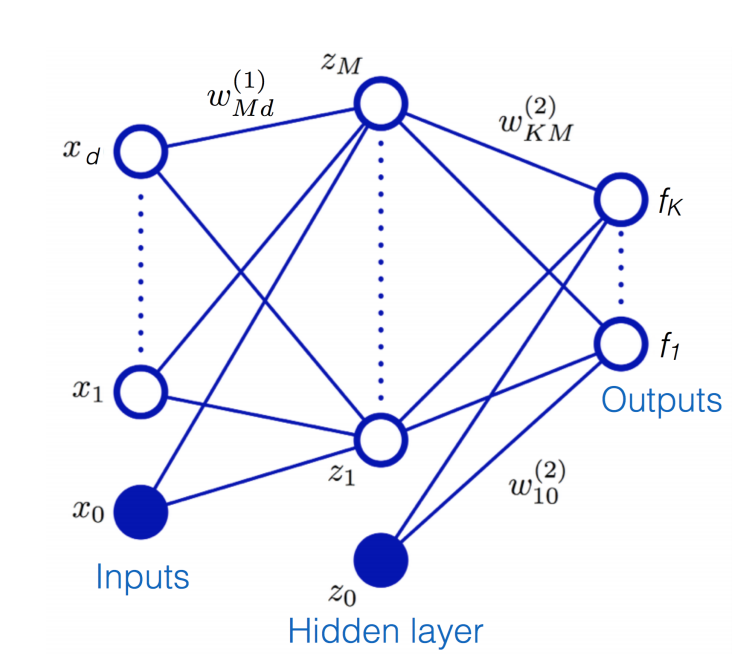
\includegraphics[width=\linewidth]{figures/neural.png}
  \caption{1-hidden layer neural networ taken from Bishop}\label{fig:neural}
\endminipage\hfill
\end{figure}
Figure 1 shows a basic neural network. The $x$ on the left is the input, with each of the $d$ dimensions acting as a separate node. These are then multiplied by the appropriate weights, added to a \textit{bias} (representing $x_0$ here), in order to obtain the \textit{activations} $a_j$ for $1\le j\le M$. These activations are then put through some non-linear map, in this case the sigmoid function, to obtain the values at the first hidden layer $z_j$. Mathematically, this looks like:
$$a_j^{(1)} = \sum_{i=1}^d w_{ji}^{(1)}x_i+w_{j0}^{(1)}$$
$$z_j = g(a_j^{(1)}) = \frac{1}{1 + e^{-a_j^{(1)}}}$$

To arrive at a simple one-hidden-layer neural network, we do this all over again, using our previous hidden layer node values (our $z_j$) instead of our inputs $x_i$ as the inputs to the second layer. Again, we add a bias feature. The equations for this layer are analogous:
$$a_k^{(2)} = \sum_{j=1}^d w_{kj}^{(2)}x_j+w_{k0}^{(1)}$$
$$f_k = g(a_k^{(2)}) = \frac{1}{1 + e^{-a_k^{(2)}}}$$

In this paper, we will consider a loss function in the form of a negative log likelihood, taking the form:
$$\ell(w) = \frac{1}{N}\sum_{i=1}^N\sum_{k=1}^K\left[-y_k^{(i)}\log(h_k(x^{(i)},w))-(1-y_k^{(i)})\log(1-h_k(x^{(i)},w))\right]$$
where $f_k=h_k$ and $y_k$ is a $K$-dimensional one-hot vector with all 0 values except for a 1 in the $k$th dimension. If we optimize this directly, however, we will often overfit to the training data (of which we have $n$ samples from $x^{(1)}$ to $x^{(n)}$ - we distinguish these from $x_i$, which are the features of one particular sample that we will consider at a time). Thus, we add a regularization term on the weights $w^{(1)}$ and $w^{(2)}$, so that we try to minize:
$$J(w) = \ell(w)+\lambda(||w^{(1)}||_F^2+||w^{(2)}||_F^2)$$
To do this, we can use our gradient descent methods from previous examinations of regression and classification; in this scenario, we want $\nabla_{w_1}J(w)$ and $\nabla_{w_2}J(w)$, which we can calculate analytically. First we compute:
$$\frac{\partial J(w)}{\partial h_k(x^{(i)},w)}=-\frac{y_k^{(i)}}{h_k(x^{(i)},w)}+\frac{1-y_k^{(i)}}{1-h_k(x^{(i)},w)}+2\lambda(||w^{(1)}||+||w^{(2)}||)$$
From the lecture notes, we have an expression for $\nabla_{w^{(2)}_k}J(w)$:
\begin{align*}
\nabla_{w^{(2)}_k}J(w)&=\frac{\partial J(w)}{\partial h_k(x^{(i)},w)}(\tilde{g}'(a_k^{(2)}))\textbf{z}\\
&=\frac{\partial J(w)}{\partial h_k(x^{(i)},w)}\frac{a_k^{(2)}}{e^{a_k^{(2)}}+1}\textbf{z}
\end{align*}
and this can be implemented with gradient descent and back-propagation to minimize the error. Similarly, we can calculate $\nabla_{w_1}J(w)$. First we let
$$\frac{\partial J(w)}{\partial a_k^{(2)}}=\frac{\partial J(w)}{\partial h_k(x^{(i)},w)}\frac{a_k^{(2)}}{e^{a_k^{(2)}}+1}=\delta_k^{(2)}$$
so that
$$\nabla_{w^{(2)}_k}J(w)=\delta_k^{(2)}\textbf{z}$$
Then, if we keep applying the chain rule like we did previously for $\nabla_{w^{(2)}_k}J(w)$, we'll get:
$$\nabla_{w^{(1)}_j}J(w)=\left(\frac{\partial J(w)}{\partial a_j^{(1)}}\right)\left(\nabla_{w^{(1)}_k}a_j^{(1)}\right)$$
where
\begin{align*}
\frac{\partial J(w)}{\partial a_j^{(1)}}&=\sum_{k=1}^K\left(\frac{\partial J(w)}{\partial a_k^{(2)}}\right)\left(\frac{\partial a_k^{(2)}}{\partial a_j^{(1)}}\right)\\
&=\sum_{k=1}^K\delta_k^{(2)}\cdot w_{kj}^{(2)}\cdot g'(a_j^{(1)})\\
&=\sum_{k=1}^K\delta_k^{(2)}\cdot w_{kj}^{(2)}\cdot \frac{a_j^{(1)}}{e^{a_j^{(1)}}+1} = \delta_j^{(1)}
\end{align*}
When we combine everything, we now have
$$\nabla_{w^{(1)}_j}J(w)=\delta_j^{(1)}\textbf{x}.$$

\section{Applications}
First, we can investigate the use of our neural network in classifying toy data. The dataset is separated into three different classes, and we are given training, validation, and test data for our model. We use cross-validation to help us optimize the number of hidden nodes, and we also test both batch and stochastic gradient descent to help us find the optimal parameters. We can initialize our parameters with $w^{(1)}_{ij}$ and $w^{(2)}_{jk}$ set randomly between 0 and 1 for all $i,j,k$ and $M=1,2,5,10$. $d$ and $K$ are determined by the input vector and the number of ``groups'' we wish to classify into. Running our gradient descents to train the neural nets, we can then plot approximate classification boundaries that the neural net reveals, as shown in Figures 2 - 5.\\

The best value of $M$, the number of hidden layers, we obtained was $M=5$ with an accuracy of $99\%$ for stochastic gradient descent. Results for the batch gradient descent matched, but the convergence was slower. The best value of $\lambda$ was 0 in both cases. We also tested our implementation on the second toy data set, which was very similar to the first - the only real difference was that the groups were less tightly clustered and it was not as easy to get near-perfect separation.\\

In addition, we tested our model on real-life MNIST data, a well-known corpus of handwritten digits from 0-9 that are often used as a benchmark for classification algorithms. This dataset that we're working with, however, only includes points with classes 1 - 6. The whole process is the same as with the toy data, just that we're working with more parameters and many more dimensions. We varied the number of hidden nodes $M$ from 5 to 100, the tradeoff regularization parameter $\lambda$ between 0.001 and 0.005, the step size of the gradient descent between 0.1 and 0.5, as well as experimented between normal gradient descent and stochastic gradient descent. For the last two parameters, we quickly concluded that in all cases a step size of .2 was approximately optimal, and that stochastic gradient descent converged much more quickly, so we stuck with those parameters while varying the rest. Across this body of tests, we obtained the cross-validation accuracies described in Table 1.\\

Our choice of parameters ended up being reasonably stable in producing passable accuracies (around $90\%$, depending on the stochastic initial parameters) and matches - we tended to favor a value of $M$ around 25, $\lambda=0.001$, and as mentioned previously, a step size of 0.2. Finally, there was no appreciable difference between the performance of batch gradient descent and stochastic gradient descent (although SGD converged significantly faster, so it is preferred).
\pagebreak

\begin{figure}[!htb]
\minipage{0.49\textwidth}
  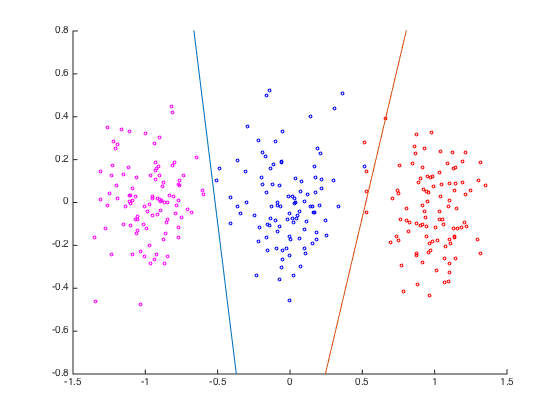
\includegraphics[width=\linewidth]{figures/batch_lambda0_toy.png}
  \caption{\texttt{toy\_1 lambda\_0 batch}}\label{fig:gradDifQ}
\endminipage\hfill
\minipage{0.49\textwidth}
  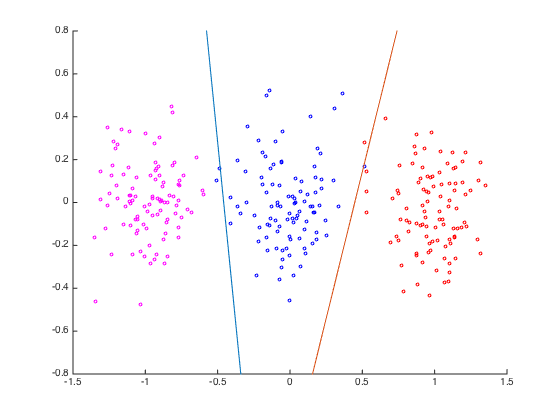
\includegraphics[width=\linewidth]{figures/batch_lambda1_toy.png}
  \caption{\texttt{toy\_1 lambda\_.05 batch}}\label{fig:gradDifN}
\endminipage\hfill
\minipage{0.49\textwidth}
  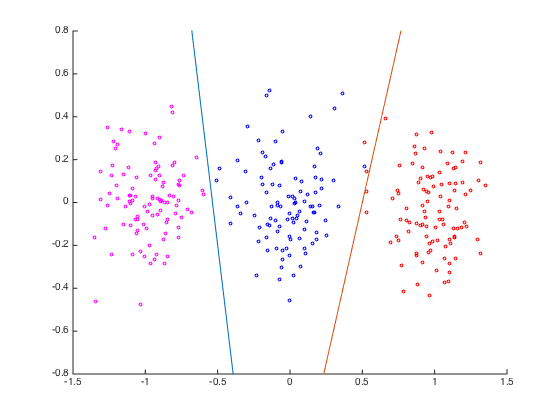
\includegraphics[width=\linewidth]{figures/sgd_lambda0_toy.png}
  \caption{\texttt{toy\_1 lambda\_0 sgd}}\label{fig:gradDifSs}
\endminipage\hfill
\minipage{0.49\textwidth}
  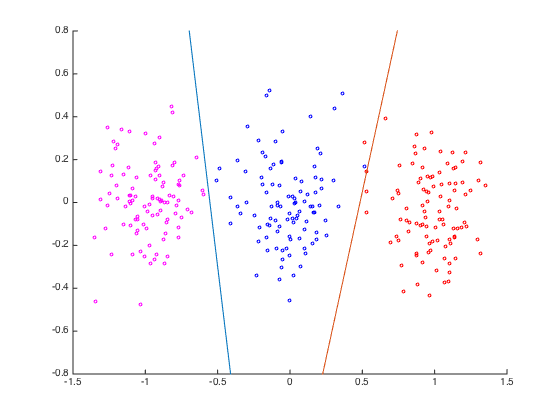
\includegraphics[width=\linewidth]{figures/sgd_lambda1_toy.png}
  \caption{\texttt{toy\_1 lambda\_.05 sgd}}\label{fig:gradDifS}
\endminipage
\end{figure}

\begin{table}[!htb]
\centering
\caption{Varying $M$ and $\lambda$ to calculate accuracy}
\label{my-label}
\begin{tabular}{rll}
M   & $\lambda$ & cross-validation accuracy \\
5   & .005    & 15.6\%   \\
5   & .001    & 17.0\%   \\
10  & .005    & 18.4\%   \\
10  & .001    & 17.9\%   \\
20  & .005    & 84.8\%   \\
20  & .001    & 83.4\%   \\
25  & .005    & 90.2\%   \\
25  & .001    & 90.6\%   \\
40  & .005    & 87.3\%   \\
40  & .001    & 86.9\%   \\
100 & .005    & 20.1\%   \\
100 & .001    & 19.2\%  
\end{tabular}
\end{table}

\pagebreak
\pagebreak

The choice of parameters is reasonable given the problem. The more data we have, in general the more complex the parameters will be in an attempt to fit all the data. However, this is balanced by the $\lambda$ that seeks to prevent overfitting via regularization of the neural net weights. Also, $M$ represents a lower-dimensional representation of the entire dataset, so it makes sense for $M$ to be some relatively small fraction of $n$, the number of training points. In this case, $n$ = 500, while our optimal $M$ was 25 - a very reasonable ratio for feature compression.
\end{document}






